\documentclass{article}
\usepackage[
				pdftex,
				colorlinks=true,
				bookmarksnumbered=true,
				bookmarksopen=true,
				bookmarksopenlevel=3,
				pdfstartview=FitP,
				urlcolor=blue,
			]{hyperref}
\pdfinfo{
			/Title(Esercitazione di Laboratorio: Oscilloscopio Digitale)
			/Author(Coa Giulio, Licastro Dario, Montano Alessandra)
		}
\usepackage[italian]{babel}
\usepackage{geometry,titling,mdsymbol,stmaryrd,graphicx,subcaption,amsmath}
\graphicspath{{./Image/}}
\renewcommand\maketitlehooka{
								\null
								\mbox{}
								\vfill
							}
\renewcommand\maketitlehookd{
								\vfill
								\null
							}
\title{
		\begin{center}
			Esercitazione di Laboratorio:
		\end{center}
		\newline
		\begin{center}
			Oscilloscopio Digitale
		\end{center}
	}
\author{
			Coa Giulio
			\and
			Licastro Dario
			\and
			Montano Alessandra
		}
\begin{document}
	%-----------------------------------------------------------------------------
	%  TITLE
	%-----------------------------------------------------------------------------
	\begin{titlingpage}
		\maketitle
	\end{titlingpage}
	\newpage
	%-----------------------------------------------------------------------------
	%  PURPOSE OF THE EXPERIENCE
	%-----------------------------------------------------------------------------
	\section{Scopo dell'esperienza}
		Lo scopo di questa esercitazione è stato misurare l'ampiezza e la frequenza di forme d’onda, prodotte da un generatore di segnali, tramite l’uso di un oscilloscopio; in particolare le fasi dell'esercitazione consistevano in:
		\begin{itemize}
			\item Misurazione dell'ampiezza e della frequenza del segnale.
			\item Misurazione del tempo di salita del segnale.
			\item Verifica del fenomeno dell’aliasing.
		\end{itemize}
	%-----------------------------------------------------------------------------
	%  INSTRUMENTATION USED
	%-----------------------------------------------------------------------------
	\section{Strumentazione utilizzata}
		La strumentazione usata durante l'esercitazione è:
		\begin{center}
			\begin{tabular}{ |c|c|c| }
				\hline
				\multirow{\textbf{Strumento}}	 & \textbf{Marca e Modello} & \textbf{Caratteristiche} \\
				\hline
				\multirow{Multimetro}			 & Agilent 34401A			& \\
				\multirow{Oscilloscopio}		 & Rigol DS1054Z			& 4 canali, \\
												 &							& $ B = 50 \, \mathrm{MHz} $, \\
												 &							& $ f_{\mathrm{c}} = 1 \, \mathrm{G\frac{Sa}{s}} $, \\
												 &							& $ R_{\mathrm{i}} = 1 \, \mathrm{M\Omega} $, \\
												 &							& $ C_{\mathrm{i}} = 13 \, \mathrm{pF} $, \\
												 &							& $ 12 \, \mathrm{Mbps} $ di profondità di memoria \\
				\multirow{Generatore di segnali} & Rigol DG1022				& 2 canali, \\
												 &							& $ f_{\mathrm{uscita}} = 20 \, \mathrm{MHz} $, \\
												 &							& $ Z_{\mathrm{uscita}} = 50 \, \mathrm{\Omega} $ \\
				\multirow{Sonda}				 & Rigol PVP215				& $ B = 35 \, \mathrm{MHz} $, \\
												 &							& $ V_{\mathrm{nominale}} = 300 \, \mathrm{V} $, \\
												 &							& $ L_{\mathrm{cavo}} = 1.2 \, \mathrm{m} $, \\
												 &							& $ R_{\mathrm{s}} = 1 \, \mathrm{M\Omega} $, \\
												 &							& Intervallo di pensazione: $ 10 \div 25 \, \mathrm{pF} $ \\
				\multirow{Cavi coassiali}		 &							& Capacità dell'ordine dei $ 80 \div 100 \, \mathrm{p\frac{F}{m}} $ \\
				\multirow{Connettori}			 &							& \\
				\hline
			\end{tabular}
		\end{center}
	%-----------------------------------------------------------------------------
	%  THEORETICAL PREMISES
	%-----------------------------------------------------------------------------
	\section{Premesse teoriche}
		\subsection{Incertezza sulla misura dell'oscilloscopio}
			La misura del valore di un segnale tramite l’oscilloscopio (sia esso l'ampiezza, la frequenza, il periodo, etc.) presenta un'incertezza che dipende, principalmente, da due fattori:
			\begin{itemize}
				\item l’incertezza strumentale introdotta dall’oscilloscopio (ricavabile dal manuale).
				\item l’incertezza di lettura dovuta all’errore del posizionamento dei cursori.
			\end{itemize}
			Quest’ultima incertezza deriva dal fatto che il segnale visualizzato non ha uno spessore nullo sullo schermo.
		\subsection{Valore efficace}
			Il valore efficace di un segnale periodico rappresenta il valore che un segnale continuo dovrebbe avere per ottenere la stessa potenza media; esso è definito come:
			\newline
			\begin{center}
				$ V_{\mathrm{eff}} = \mathrm{\sqrt{\frac{1}{T} \int_{0}^{T} V(t)^{2} \, dt}} $
			\end{center}
			\newline
			Per i segnali sinusoidali del tipo
			\newline
			\begin{center}
				$ V = A \cdot \mathrm{\sin(\overline{\omega} \cdot t)} $
			\end{center}
			il valore efficace corrisponde a
			\newline
			\begin{center}
				$ V_{\mathrm{eff}} = \mathrm{\frac{A}{\sqrt{2}}} $
			\end{center}
		\subsection{Tempo di salita}
			Il tempo di salita di un segnale è definito come il tempo che il segnale impiega per passare dal $ 10\% $ al $ 90\% $ della sua ampiezza.
			\newline
			Nel caso in cui si stia analizzando un filtro passa-basso, vale la seguente la relazione che collega la banda del filtro ($ B $) e il tempo di salita del segnale ($ t_{\mathrm{salita}} $):
			\newline
			\begin{center}
				$ B \cdot t_{\mathrm{salita}} = 0.35 $
			\end{center}
			\newline
			\begin{scriptsize}
				\textbf{N.B.} Questa relazione vale solo per gli oscilloscopi analogici; nel caso di un oscilloscopio digitale la costante deve essere tratta dal manuale. 
			\end{scriptsize}
			\newline
			\newline
			Inoltre, nel caso si voglia misurare il tempo di salita tramite un oscilloscopio, vale la relazione
			\newline
			\begin{center}
				$ t_{\mathrm{salita}}^{2} = t_{\mathrm{salitaEffettivo}}^{2} + t_{\mathrm{oscilloscopio}}^{2} $
			\end{center}
			\newline
			dove $ t_{\mathrm{oscilloscopio}} $ rappresenta il tempo di salita introdotto dall’oscilloscopio.
		\subsection{Sonda}
			La sonda è un particolare cavo coassiale che presenta un'estremità capace di effettuare delle mi-
			\newline
			surazioni.
			\newline
			Quando si usano dei classici cavi coassiali BNC-BNC al fine di collegare il circuito, su cui effettuare le misure, all'oscilloscopio, si sta inserendo in parallelo al circuito un condensatore di capacità ($ C_{\mathrm{c}} $) pari a quella del cavo.
			\begin{figure}[h!]
				\centering
				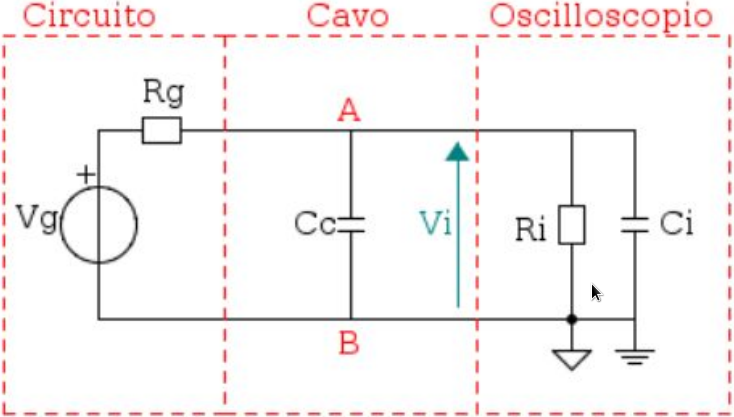
\includegraphics[scale=0.4]{theveninCavoDSO}
				\caption{Circuito analizzato collegato all'oscilloscopio tramite un cavo coassiale BNC-BNC.}
				\label{fig:theveninCavoDSO}
			\end{figure}
			\newpage
			In questo caso, l’oscilloscopio si comporta, in ingresso, come un filtro passa-basso con una frequenza di taglio ($ f = \frac{1}{2\pi R_{i} (C_{s} + C_{i})} $). L'uso di una sonda per misurare delle grandezze in un circuito, si può vedere come l'inserimento di un condensatore in serie al circuito.
			\begin{figure}[h!]
				\centering
				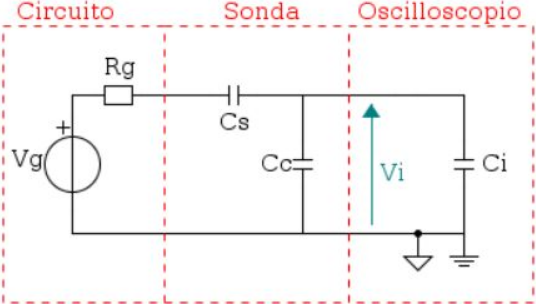
\includegraphics[scale=0.4]{theveninSondaDSOCircuito}
				\caption{Circuito analizzato collegato all'oscilloscopio tramite una sonda.}
				\label{fig:theveninSondaDSOCircuito}
			\end{figure}
			\newline
			L'introduzione di questo condensatore comporta un calo della capacità equivalenti vista all'ingresso del circuito ($ \mathrm{\frac{C_{s} (C_{c} + C_{i})}{C_{s} + C_{c} + C_{i}} \ll C_{c} + C_{i}} $), ovvero una riduzione della frequenza del polo ($ f_{\mathrm{polo}} = \frac{1}{2\pi R_{i} (C_{s} + C_{i})} $); ciò porta ad una perdita d'informazioni in bassa frequenza.
			\newline
			Al fine di evitare tale perdita d'informazioni, si pone, in parallelo al condensatore, una resistenza.
			\begin{figure}[h!]
				\centering
				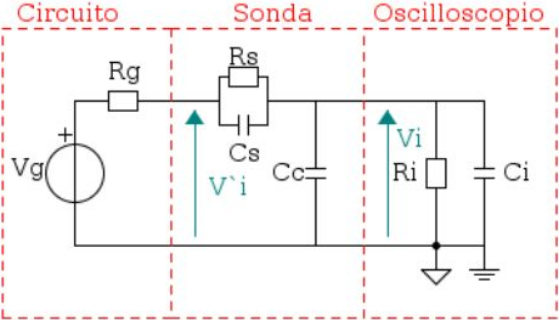
\includegraphics[scale=0.4]{theveninSondaDSOResistenza}
				\caption{Circuito analizzato collegato all'oscilloscopio tramite una sonda.}
				\label{fig:theveninSondaDSOResistenza}
			\end{figure}
			\newline
			Tale resistenza comporta la presenza di uno zero, oltre al polo precedentemente detto.
			\begin{figure}[h!]
				\centering
				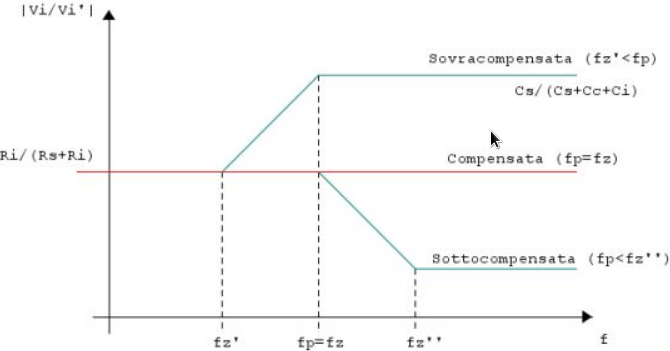
\includegraphics[scale=0.4]{sondaBode}
				\caption{Diagramma di Bode della funzione di trasferimento del circuito.}
				\label{fig:sondaBode}
			\end{figure}
			\newpage
			A seconda dell'elevata o della bassa compensazione della sonda, il segnale sarà distorto verso l'alto o verso il basso.
			\begin{figure}[h!]
				\centering
				\begin{subfigure}{0.4\textwidth}
					\centering
					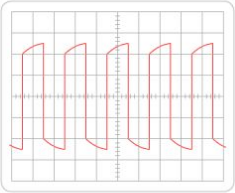
\includegraphics[scale=0.5]{sondaSegnaleSottocompensato}
					\caption{Sonda sottocompensata.}
				\end{subfigure}
				\begin{subfigure}{0.4\textwidth}
					\centering
					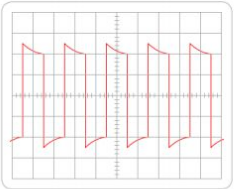
\includegraphics[scale=0.5]{sondaSegnaleSovracompensato}
					\caption{Sonda sovracompensata.}
				\end{subfigure}
				\caption{Visualizzazione del segnale al variare della compensazione della sonda.}
				\label{fig:sondaSegnaleNonCompensato}
			\end{figure}
			\newline
			La sonda risulta compensata quando la frequenza del polo coincide con la frequenza dello zero; ciò avviene quando $ R_{\mathrm{s}} C_{\mathrm{s}} = R_{\mathrm{i}} (C_{\mathrm{c}} + C_{\mathrm{i}})} $. La sonda presenta un opportuno trimmer che influenza il valore di $ R_{\mathrm{s}} $ e permette la compensazione. Al fine di verificare se la sonda è compensata si esegue un confronto con un segnale noto.
			\begin{figure}[h!]
				\centering
				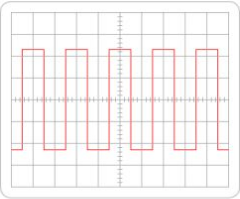
\includegraphics[scale=0.5]{sondaSegnaleCompensato}
				\caption{Sonda compensata.}
				\label{fig:sondaSegnaleCompensato}
			\end{figure}
		\subsection{Aliasing}
			L’aliasing è un fenomeno che si verifica quando non viene adoperata un’adeguata frequenza di campionamento per il segnale di ingresso, ovvero quando non viene rispettato il teorema del cam-
			\newline
			pionamento e si sottocampiona il segnale; ciò comporta una visualizzazione errata del segnale (perdita d'informazioni sul segnale) dovuta alla sovrapposizione di due ripetizioni del segnale.
			\begin{figure}[h!]
				\centering
				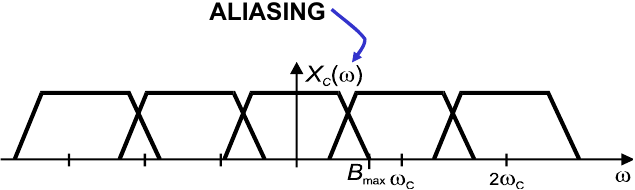
\includegraphics[scale=0.4]{aliasing}
				\caption{Aliasing nel dominio delle frequenze.}
				\label{fig:aliasing}
			\end{figure}
			\newpage
			Al fine di evitare questo fenomeno, si usano dei filtri passa-basso particolari detti, appunto, filtri anti-aliasing. Nel caso in cui ci si ritrovi in tale situazione, a volte, basta regolare la base tempi, in modo da poter visualizzare il segnale correttamente.
			\subsubsection{Aliasing percettivo}
				In alcune occasioni è possibile che si verifichi il fenomeno dell’aliasing percettivo, ovvero la non corretta visione da parte dell’operatore della forma d’onda rappresentata sull’oscilloscopio, nonostante quest’ultima sia rappresentata correttamente.
	%-----------------------------------------------------------------------------
	%  LABORATORY EXPERIENCE
	%-----------------------------------------------------------------------------
	\section{Esperienza in laboratorio}
		\subsection{Misurazione del valore efficace e della frequenza del segnale}
			\subsubsection{Operazioni preliminari}
				Abbiamo regolato il generatore di segnali in modo da visualizzare un segnale sinusoidale di ampiezza $ V_{\mathrm{pp}} = 1 \, \mathrm{V} $ e frequenza $ f = 1 \, \mathrm{kHz} $; successivamente abbiamo collegato il generatore di segnali all'oscilloscopio tramite un cavo coassiale BNC-BNC al fine di visualizzare la forma d'onda.
				\begin{figure}[h!]
					\centering
					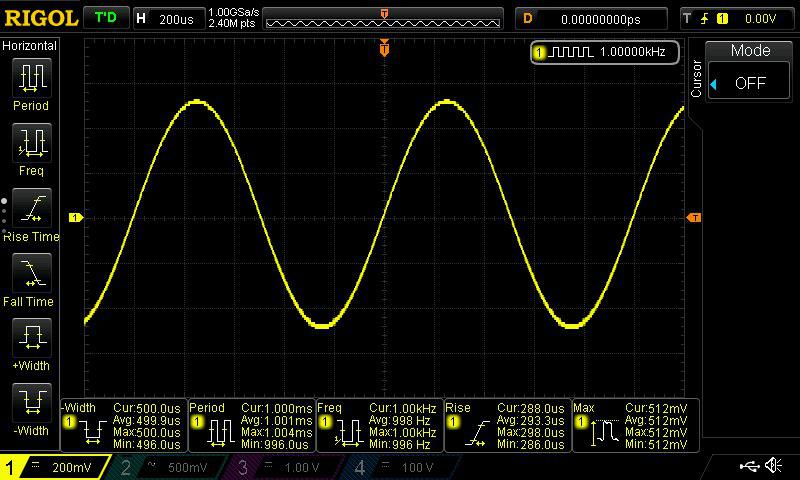
\includegraphics[scale=0.3]{segnalePuro}
					\caption{Segnale sinusoidale di ampiezza $ V_{\mathrm{pp}} = 1 \, \mathrm{V} $ e frequenza $ f = 1 \, \mathrm{kHz} $.}
					\label{fig:segnalePuro}
				\end{figure}
			\subsubsection{Misurazione del valore efficace del segnale}
				Abbiamo determinato, tramite l'uso dei cursori, l'ampiezza del segnale e, successivamente, l'incertezza di misura. Infine, si è determinato il valore efficace del segnale e la sua incertezza.
				\begin{figure}[h!]
					\centering
					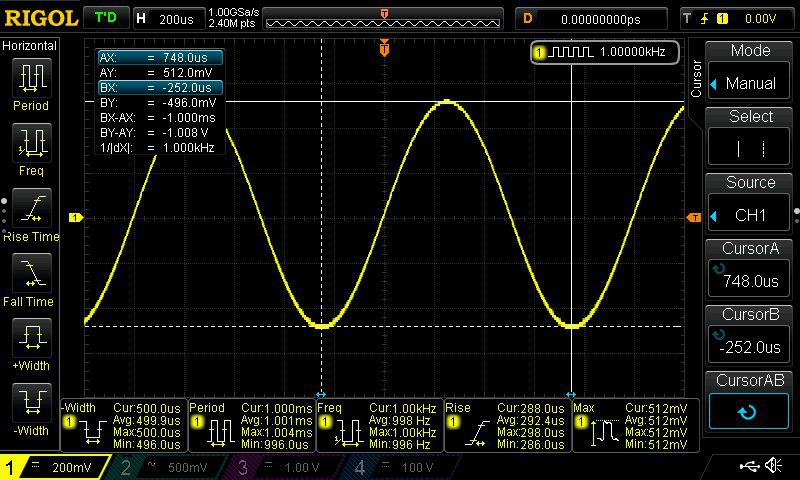
\includegraphics[scale=0.3]{segnaleMisure}
					\caption{Misurazione dell'ampiezza e della frequenza del segnale.}
					\label{fig:segnaleMisure}
				\end{figure}
			\subsubsection{Misurazione della frequenza del segnale}
				Abbiamo determinato, tramite l'uso dei cursori, il periodo del segnale e, successivamente, l'incertezza di misura. Infine, si è determinato la frequenza del segnale e la sua incertezza (si veda la figura~\ref{fig:segnaleMisure}).
			\subsubsection{Verifica col multimetro}
				Abbiamo misurato, tramite l'uso del multimetro, sia il valore efficace sia la frequenza del segnale, procedendo, poi, al calcolo delle relative incertezze di misura.
		\subsection{Misurazione del tempo di salita del segnale}
			\subsubsection{Operazioni preliminari}
				Abbiamo regolato il generatore di segnali in modo da visualizzare un segnale ad onda quadra di ampiezza $ V_{\mathrm{pp}} = 1 \, \mathrm{V} $ e frequenza $ f = 1 \, \mathrm{kHz} $ (si veda la figura~\ref{fig:segnalePuro}).
			\subsubsection{Tempo di salita in condizioni di adattamento di impedenza}
				Abbiamo inserito in parallelo all'ingresso dell'oscilloscopio un terminatore di valore pari a $ 50 \, \mathrm{\Omega} $, collegato tramite un connettore a $ \mathrm{\downassert} $. In questo modo, l'oscilloscopio mostra al cavo caoassiale BNC-BNC un'impedenza d'ingresso di $ 50 \, \mathrm{\Omega} $.
				\begin{figure}[h!]
					\centering
					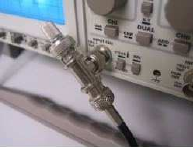
\includegraphics[scale=0.7]{connettoreAT}
					\caption{Connessione della resistenza da $ 50 \, \mathrm{\Omega} $ in parallelo all'ingresso dell'oscilloscopio.}
					\label{fig:connettoreAT}
				\end{figure}
				\newpage
				Successivamente abbiamo regolato l'oscilloscopio in modo da visualizzare il fronte di salita del segnale e abbiamo eseguito la misurazione, tramite i cursori, del tempo di salita.
				\begin{figure}[h!]
					\centering
					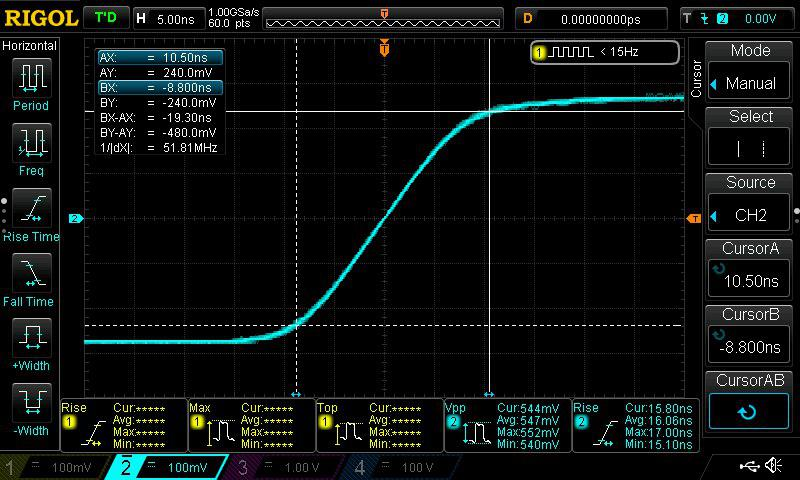
\includegraphics[scale=0.3]{tempoSalitaAdattamentoImpedenza}
					\caption{Misurazione del tempo di salita di un segnale ad onda quadra di ampiezza $ V_{\mathrm{pp}} = 1 \, \mathrm{V} $ e frequenza $ f = 1 \, \mathrm{kHz} $.}
					\label{fig:tempoSalitaAdattamentoImpedenza}
				\end{figure}
				\newline
				Questa misurazione presenta un errore sistematico dovuto alla banda dell'oscilloscopio, per cui abbiamo calcolato tale errore per poter stabilire se la misura effettuata andasse corretta o meno al fine di ottenere il reale tempo di salita.
			\subsubsection{Tempo di salita con generatore ad alta impedenza: uso della sonda compensata}
				Abbiamo inserito in serie all'ingresso dell'oscilloscopio, o, a seconda dei punti di vista, all'uscita del generatore di segnali, una resistenza di valore pari a $ 1 \, \mathrm{k\Omega} $, collegata tramite una coppia di cavi BNC-coccodrillo (abbiamo collegato un cavo al generatore di segnali e un cavo all'oscilloscopio; successivamente abbiamo unito tra di loro i coccodrilli rappresentanti il polo negativo e abbiamo posto quelli rappresentanti il polo positivo ai capi della resistenza). In questo modo, il generatore di segnali presenta una resistenza interna pari a $ 1'050 \, \mathrm{\Omega} $, di cui $ 50 \, \mathrm{\Omega} $ dovuti alla resistenza interna del generatore di segnali; a seguito di ciò, il circuito equivalente è diventato
				\begin{figure}[h!]
					\centering
					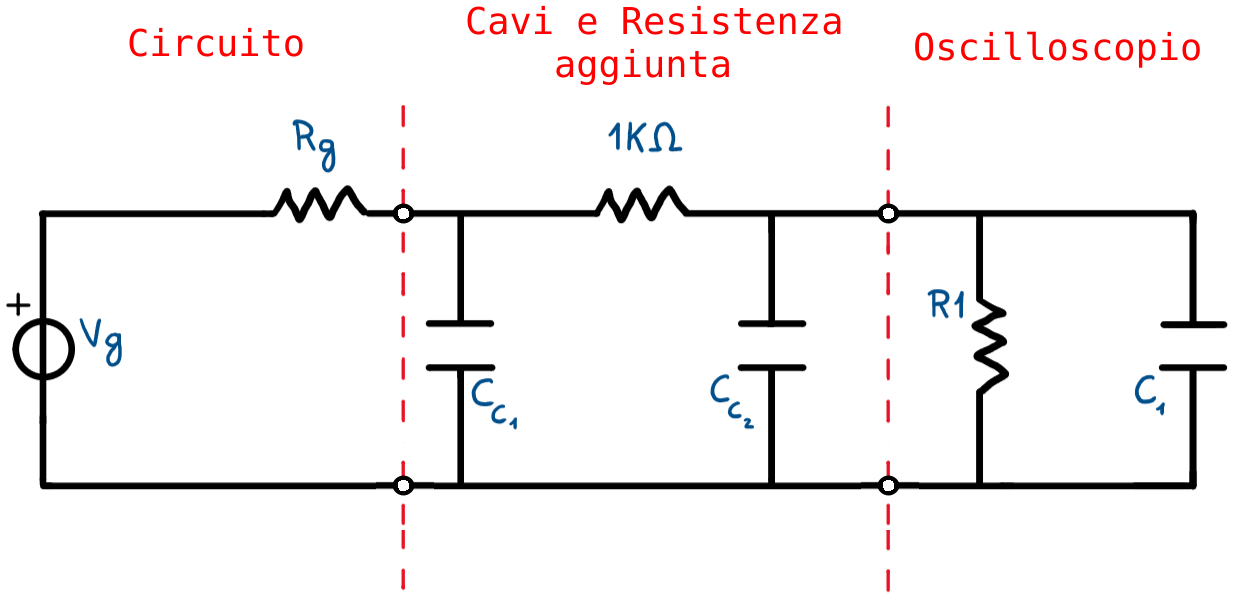
\includegraphics[scale=0.5]{circuitoResistenzaSerieCavo}
					\caption{Connessione, tramite il cavo, della resistenza da $ 1 \, \mathrm{k\Omega} $ in serie all'uscita del generatore di segnali.}
					\label{fig:circuitoResistenzaSerieCavo}
				\end{figure}
				\newpage
				Abbiamo, poi, proceduto al calcolo, sia teorico sia tramite i cursori, del nuovo tempo di salita del segnale, soggetto all'effetto del filtro passa-basso costituito dalla resistenza interna del generatore di segnali ($ R_{\mathrm{g}} $), dalla capacità del cavo ($ C_{\mathrm{c}} $) e dalla capacità d'ingresso dell'oscilloscopio ($ C_{\mathrm{i}} $).
				\begin{figure}[h!]
					\centering
					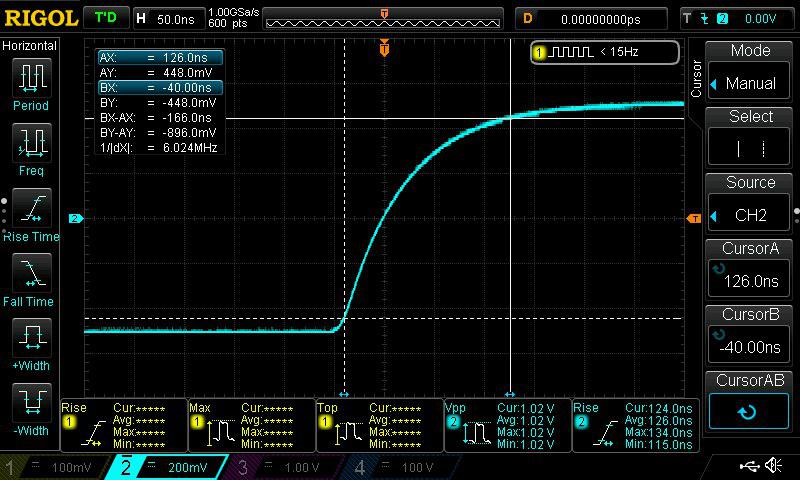
\includegraphics[scale=0.3]{tempoSalitaAltaImpedenza}
					\caption{Misurazione del tempo di salita del segnale dopo aver posto in serie la resistenza da $ 1 \, \mathrm{k\Omega} $.}
					\label{fig:tempoSalitaAltaImpedenza}
				\end{figure}
				\newline
				Infine, abbiamo sostituito il cavo BNC-coccodrillo che connetteva la resistenza da $ 1 \, \mathrm{k\Omega} $ all'oscilloscopio con la sonda (abbiamo collegato la testa della sonda, rappresentante il polo positivo, alla resistenza e il coccodrillo della sonda, rappresentante il polo negativo, al coccodrillo dell'altro cavo BNC-coccodrillo); in questo modo, il circuito equivalente è diventato
				\begin{figure}[h!]
					\centering
					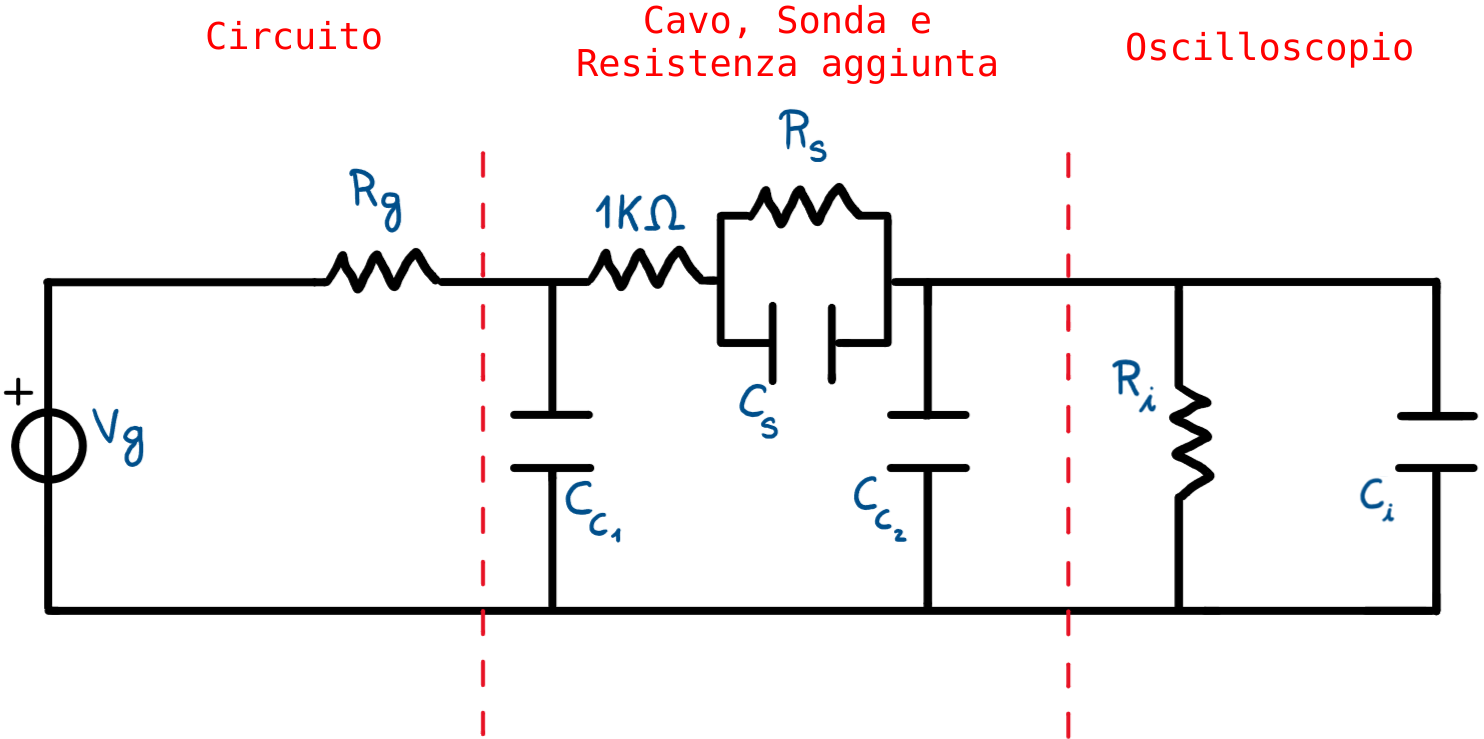
\includegraphics[scale=0.5]{circuitoResistenzaSerieSonda}
					\caption{Connessione, tramite la sonda, della resistenza da $ 1 \, \mathrm{k\Omega} $ in serie all'uscita del generatore di segnali.}
					\label{fig:circuitoResistenzaSerieSonda}
				\end{figure}
				\newpage
				A questo punto, abbiamo compensanto la sonda tramite il suo trimmer, verificandone l'effetto su un segnale ad onda quadra, e abbiamo ripetuto il procedimento effettuato al punto precedente.
				\begin{figure}[h!]
					\centering
					\begin{subfigure}{0.4\textwidth}
						\centering
						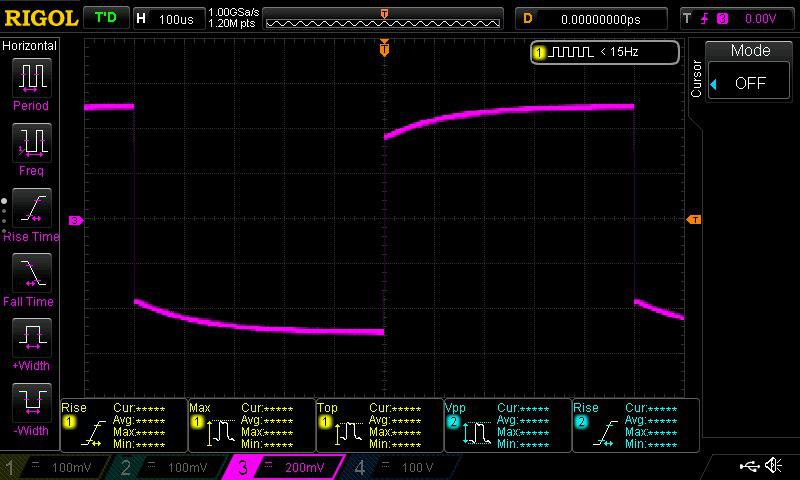
\includegraphics[scale=0.2]{tempoSalitaSondaNonCompensata}
						\caption{Segnale dopo aver sostituito il cavo BNC-BNC con la Sonda.}
					\end{subfigure}
					\begin{subfigure}{0.4\textwidth}
						\centering
						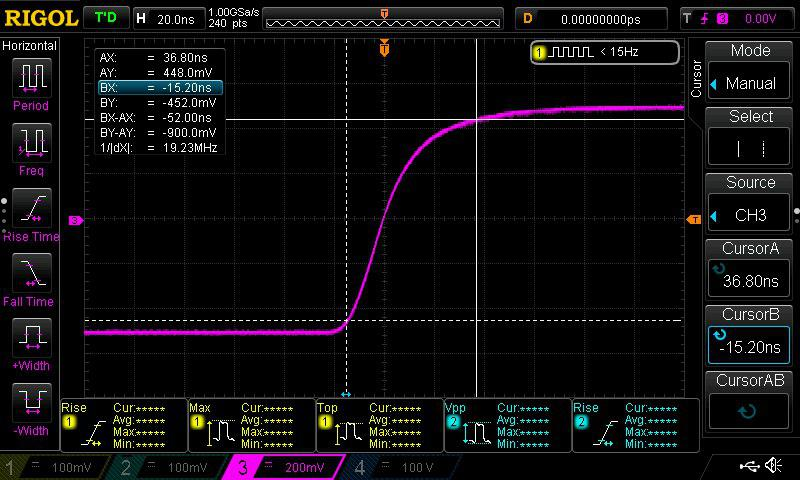
\includegraphics[scale=0.2]{tempoSalitaSondaCompensata}
						\caption{Misurazione del tempo di salita del segnale dopo aver compensato la Sonda.}
					\end{subfigure}
					\label{fig:tempoSalitaSonda}
				\end{figure}
		\subsection{Verifica del fenomeno dell’aliasing}
			\subsubsection{Operazioni preliminari}
				Abbiamo regolato il generatore di segnali in modo da visualizzare un segnale sinusoidale di ampiezza $ V_{\mathrm{pp}} = 1 \, \mathrm{V} $ e frequenza $ f = 100 \, \mathrm{kHz} $, per poi procedere al calcolo della minima frequenza di campionamento ($ f_{\mathrm{c}} $). Successivamente abbiamo verificato se essa era compatibile con la frequenza di campionamento dell'oscilloscopio, al fine di determinare se il teorema del campionamento fosse rispettato o meno. Infine abbiamo determinato, come richiesto, il numero di campioni presenti in un periodo del segnale sia analiticamente sia tramite l'uso dei cursori.
			\subsubsection{Aliasing percettivo}
				Abbiamo ridotto la velocità di scansione (nell'effettivo abbiamo ridotto la profondità della memoria e aumentato il numero di $ \mathrm{\frac{s}{div}} $) e osservato come essa influisse sulla frequenza di campionamento (comporta un calo della suddetta frequenza); successivamente abbiamo impostato la velocità di scansione in modo tale da ottenere una frequenza di campionamento $ f_{\mathrm{c}} = 1 \, \mathrm{MHz} $, ovvero abbiamo ridotto la profondità della memoria a $ 12 \, \mathrm{kSa} $, e abbiamo impostato l'oscilloscopio in DOTS MODE, ovvero senza l'interpolazione dei punti, ottenendo il seguente segnale.
				\newline
				\begin{figure}[h!]
					\centering
					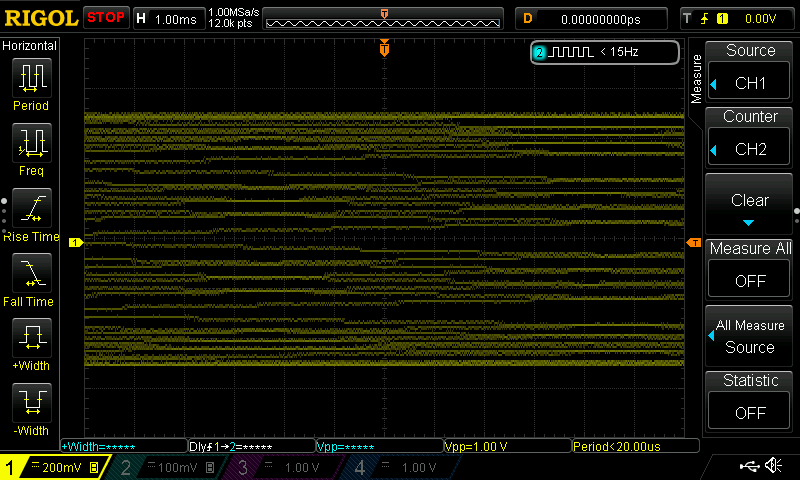
\includegraphics[scale=0.4]{aliasingPercettivo1MHz}
					\caption{Segnale a $ 100 \, \mathrm{kHz} $ affetto da aliasing percettivo.}
					\label{fig:aliasingPercettivo1MHz}
				\end{figure}
				\newline
				In questo caso il teorema del campionamento è rispettato, ma il segnale rappresentato non corrisponde ad una sinusoide in quanto viene sovracampionato (il numero di $ \mathrm{\frac{Sa}{div}} $ è troppo elevato perchè l'oscilloscopio riesca a rappresentare il segnale in maniera adeguata). Al fine di visualizzare meglio il segnale, abbiamo dovuto diminuire il numero di $ \mathrm{\frac{s}{div}} $.
				\newline
				Infine abbiamo portato la frequenza del generatore di segnali a $ 100.1 \, \mathrm{kHz} $, ottenendo il seguente segnale.
				\begin{figure}[h!]
					\centering
					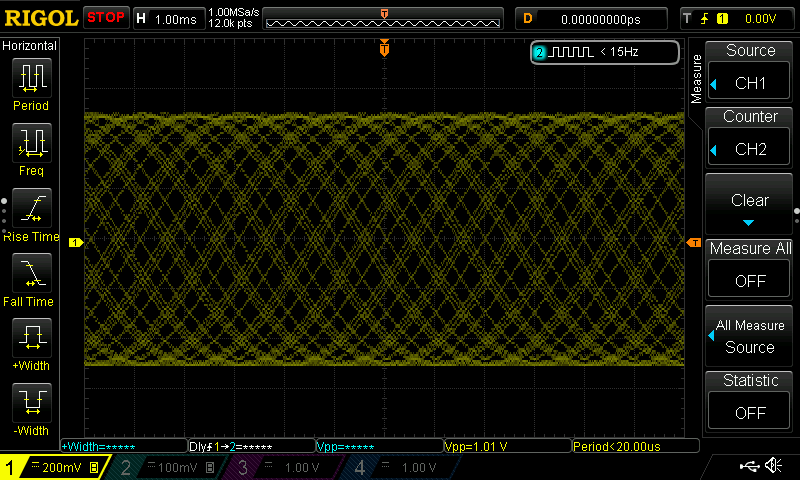
\includegraphics[scale=0.4]{aliasingPercettivo100kHz}
					\caption{Segnale a $ 100.1 \, \mathrm{kHz} $ affetto da aliasing percettivo.}
					\label{fig:aliasingPercettivo100kHz}
				\end{figure}
				\newpage
				Questo è un caso analogo al precedente, ma si distingue da esso in quanto il fenomeno dell'aliasing percettivo è "meno marcato".
			\subsubsection{Aliasing nel dominio del tempo}
				Abbiamo regolato il generatore di segnali in modo da visualizzare il segnale sinusoidale ad una frequenza $ f = 100.1 \, \mathrm{kHz} $, per poi procedere ad una riduzione della velocità di scansione fino a giungere ad una frequenza di campionamento $ f_{\mathrm{c}} = 100 \, \mathrm{kHz} $. Successivamente abbiamo misurato, tramite i cursori, la frequenza del segnale ottenenuto.
				\begin{figure}[h!]
					\centering
					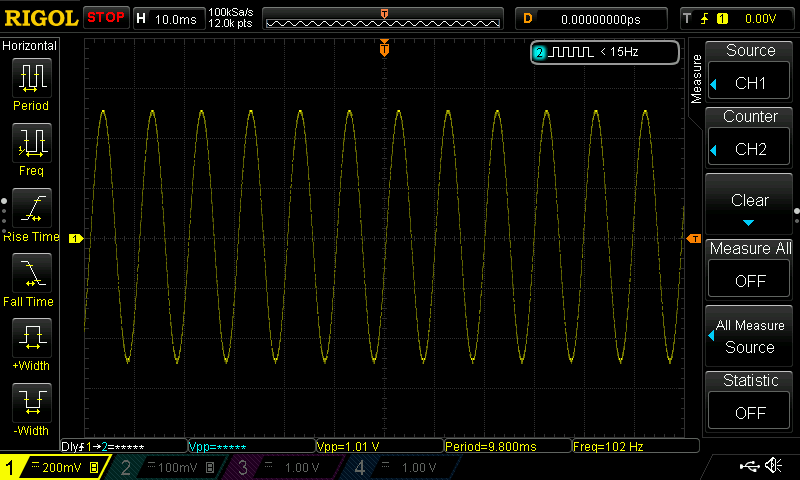
\includegraphics[scale=0.4]{aliasing100_1kHz}
					\caption{Segnale a $ 100.1 \, \mathrm{kHz} $ affetto da aliasing.}
					\label{fig:aliasing100_1kHz}
				\end{figure}
				\newpage
				In questo caso il teorema del campionamento non è rispettato; infatti, sull’oscilloscopio, viene rappresentato un segnale non statico la cui frequenza, misurata tramite i cursori, è pari a $ 102 \, \mathrm{Hz} $.
				\newline
				Infine, abbiamo riportato la frequenza del generatore di segnali a $ f = 100 \, \mathrm{kHz} $, ottenendo il seguente segnale.
				\begin{figure}[h!]
					\centering
					\begin{subfigure}{0.4\textwidth}
						\centering
						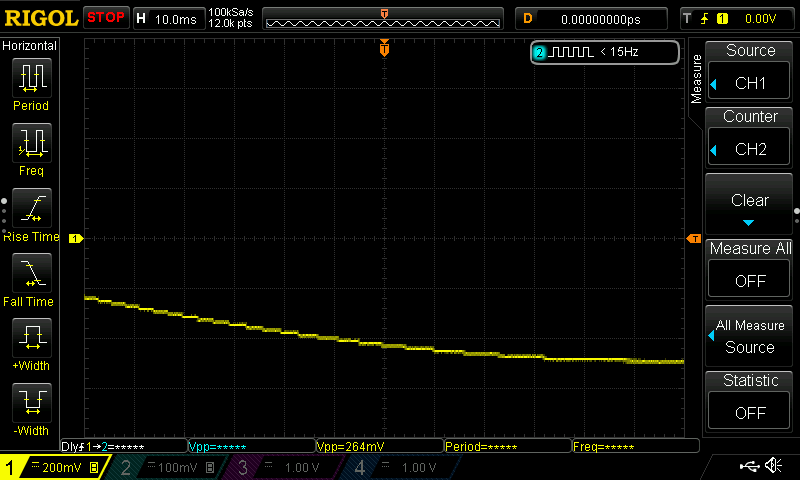
\includegraphics[scale=0.2]{aliasing100kHz_1}
					\end{subfigure}
					\begin{subfigure}{0.4\textwidth}
						\centering
						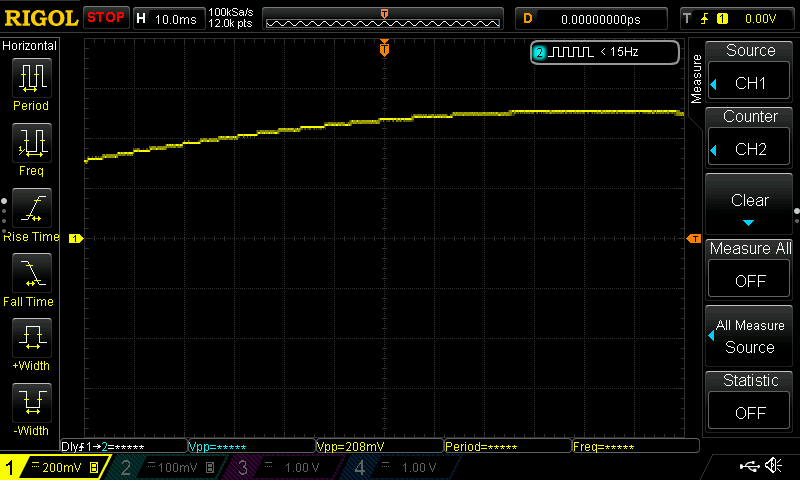
\includegraphics[scale=0.2]{aliasing100kHz_2}
					\end{subfigure}
					\newline
					\centering
					\begin{subfigure}{0.4\textwidth}
						\centering
						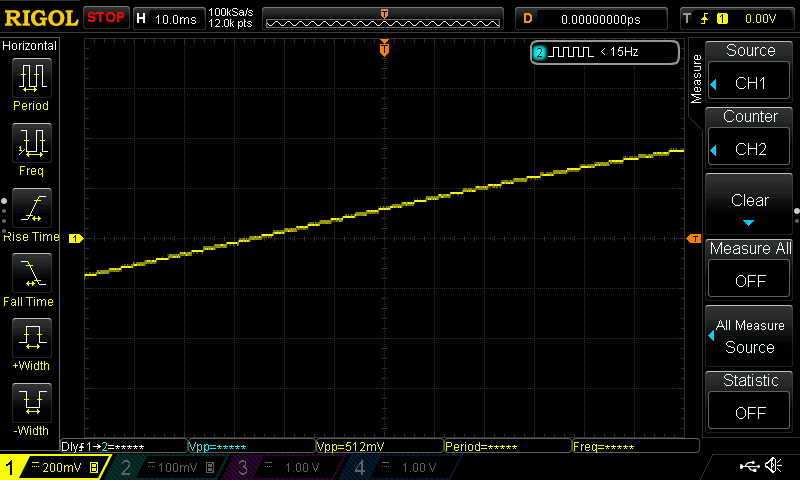
\includegraphics[scale=0.2]{aliasing100kHz_3}
					\end{subfigure}
					\caption{Segnale a $ 100 \, \mathrm{kHz} $ affetto da aliasing.}
					\label{fig:aliasing100kHz}
				\end{figure}
				\newpage
				Anche in questo caso il teorema del campionamento non viene rispettato; infatti, sull’oscilloscopio, viene visualizzato un segnale non statico, come si nota dalla sequenza d'immagini~\ref{fig:aliasing100kHz}, rappresentanti il segnale in momenti differenti, e con un periodo che non riesce ad essere rappresentato nella sua completezza.
	%-----------------------------------------------------------------------------
	%  RESULTS
	%-----------------------------------------------------------------------------
	\section{Risultati}
		\subsection{Misurazione del valore efficace e della frequenza del segnale}
			\subsubsection{Misurazione del valore efficace del segnale}
				L'incertezza relativa associata alla misurazione è pari a 
				\begin{equation*}
					\begin{split}
						\epsilon V_{\mathrm{pp}} &= \epsilon n_{\mathrm{div}} + \epsilon_{\mathrm{oscilloscopio}} = \\
												 &= \frac{\delta n_{\mathrm{div}}}{n_{\mathrm{div}}} + \frac{\delta_{\mathrm{oscilloscopio}}}{V_{\mathrm{m}}} = \\
												 &= \frac{\delta n_{\mathrm{div}}}{n_{\mathrm{div}}} + \frac{\frac{3}{100}V_{\mathrm{fs}}}{V_{\mathrm{m}}} = \\
												 &= \frac{0.2}{4} + \frac{\frac{3}{100} \cdot 500 \cdot 8}{1.01}m = \\
												 &= \frac{1}{20} + \frac{12}{101} = \\
												 &= 0.050 + 0.119 = \\
												 &= 0.169
					\end{split}
				\end{equation*}
				Da cui
				\begin{equation*}
					\begin{split}
						\delta V_{\mathrm{pp}} &= \epsilon V_{\mathrm{pp}} \cdot V_{\mathrm{pp}} = \\
											   &= 0.169 \cdot 1.01 = \\
											   &= 0.171 \, \mathrm{V}
					\end{split}
				\end{equation*}
				L'ampiezza del segnale analizzato è, quindi, pari a
				\newline
				\begin{center}
					$ V_{\mathrm{pp}} = 1.01 \pm 0.171 \, \mathrm{V} $
				\end{center}
				\newline
				Sapendo l'ampiezza del segnale, abbiamo potuto determinarne il valore efficace tramite la sua definizione ($ V_{\mathrm{eff}} = \mathrm{\frac{V_{pp}}{\sqrt{2}}} $), ottenendo
				\newline
				\begin{center}
					$ V_{\mathrm{eff}} = 714 \pm 121 \, \mathrm{mV} $
				\end{center}
				\newline
				Dove l'incertezza è stata calcolata tramite la formula
				\begin{equation*}
					\begin{split}
						\epsilon V_{\mathrm{eff}} &= \epsilon_{\mathrm{\sqrt{2}}} + \epsilon V_{\mathrm{pp}} = \\
												  &= \epsilon V_{\mathrm{pp}} = \\
												  &= 0.169
					\end{split}
				\end{equation*}
				Da cui
				\begin{equation*}
					\begin{split}
						\delta V_{\mathrm{eff}} &= \epsilon V_{\mathrm{eff}} \cdot V_{\mathrm{eff}} = \\
												&= 0.169 \cdot 714 = \\
												&= 121 \, \mathrm{mV}
					\end{split}
				\end{equation*}
			\subsubsection{Misurazione della frequenza del segnale}
				L'incertezza relativa associata alla misurazione è pari a 
				\begin{equation*}
					\begin{split}
						\epsilon T &= \epsilon n_{\mathrm{div}} + \epsilon_{\mathrm{oscilloscopio}} = \\
								   &= \frac{\delta n_{\mathrm{div}}}{n_{\mathrm{div}}} + \frac{\delta_{\mathrm{oscilloscopio}}}{T_{\mathrm{m}}} = \\
								   &= \frac{\delta_{\mathrm{n_{\mathrm{div}}}}}{n_{\mathrm{div}}} + \frac{25\mu \cdot T_{\mathrm{fs}}}{T_{\mathrm{m}}} = \\
								   &= \frac{0.2}{2} + \frac{25 \cdot 500 \cdot 8}{1.00}p = \\
								   &= \frac{1}{10} + 100n = \\
								   &= 0.100 + 100n = \\
								   &\approx 0.100
					\end{split}
				\end{equation*}
				Da cui
				\begin{equation*}
					\begin{split}
						\delta T &= \epsilon T \cdot T = \\
								 &= 0.100 \cdot 1.00m = \\
								 &= 0.100 \, \mathrm{ms}
					\end{split}
				\end{equation*}
				Il periodo del segnale analizzato è, quindi, pari a
				\newline
				\begin{center}
					$ T = 1.00 \pm 0.100 \, \mathrm{ms} $
				\end{center}
				\newline
				Sapendo il periodo del segnale, abbiamo potuto determinarne la frequenza tramite la sua definizione ($ f = \mathrm{\frac{1}{T}} $), ottenendo
				\newline
				\begin{center}
					$ f = 1.00 \pm 0.100 \, \mathrm{kHz} $
				\end{center}
				\newline
				Dove l'incertezza è stata calcolata tramite la formula
				\begin{equation*}
					\begin{split}
						\delta f &= \lvert \frac{1}{T^{2}} \rvert \cdot \delta T = \\
								 &= \lvert \frac{1}{1.00^{2}} \rvert M \cdot 0.100m = \\
								 &= 0.100 \, \mathrm{kHz}
					\end{split}
				\end{equation*}
			\subsubsection{Verifica col multimetro}
				Tramite il multimetro, abbiamo misurato il seguente valore efficace
				\newline
				\begin{center}
					$ V_{\mathrm{eff}} = 714 \pm 225 \, \mathrm{mV} $
				\end{center}
				Si può notare come il valore sia coerente con quello calcolato, ma presenti un'incertezza maggiore rispetto ad esso.
				\newline
				Abbiamo, poi, misurato la seguente frequenza
				\newline
				\begin{center}
					$ f = 999 \pm 0.0100 \, \mathrm{Hz} $
				\end{center}
				Al contrario del valore efficace, la frequenza, per quanto il risultato, presenta un'incertezza minore rispetto a quella calcolata.
		\subsection{Misurazione del tempo di salita del segnale}
			\subsubsection{Tempo di salita in condizioni di adattamento di impedenza}
				L'incertezza relativa associata alla misurazione è pari a 
				\begin{equation*}
					\begin{split}
						\epsilon t_{\mathrm{salitaMisurato}} &= \epsilon n_{\mathrm{div}} + \epsilon_{\mathrm{oscilloscopio}} = \\
														 	 &= \frac{\delta n_{\mathrm{div}}}{n_{\mathrm{div}}} + \frac{\delta_{\mathrm{oscilloscopio}}}{t_{\mathrm{salitaMisurato}}} = \\
														 	 &= \frac{\delta_{\mathrm{n_{\mathrm{div}}}}}{n_{\mathrm{div}}} + \frac{25\mu \cdot t_{\mathrm{fs}}}{t_{\mathrm{salitaMisurato}}} = \\
														 	 &= \frac{0.2}{3} + \frac{25 \cdot 500 \cdot 8}{19.3}\mu = \\
														 	 &= \frac{1}{15} + 5.18m = \\
														 	 &= 0.0667 + 5.18m = \\
														 	 &= 0.0719
					\end{split}
				\end{equation*}
				Da cui
				\begin{equation*}
					\begin{split}
						\delta t_{\mathrm{salitaMisurato}} &= \epsilon t_{\mathrm{salitaMisurato}} \cdot t_{\mathrm{salitaMisurato}} = \\
														   &= 0.0719 \cdot 19.3n = \\
														   &= 1.39 \, \mathrm{ns}
					\end{split}
				\end{equation*}
				Il tempo di salita del segnale analizzato è, quindi, pari a
				\newline
				\begin{center}
					$ t_{\mathrm{salitaMisurato}} = 19.3 \pm 1.39 \, \mathrm{ns} $
				\end{center}
				\newline
				Come detto in precedenza, questa misurazione è affetta da un errore sistematico del valore di
				\begin{equation*}
					\begin{split}
						t_{\mathrm{oscilloscopio}} &= \frac{0.35}{B} = \\
												   &= \frac{0.35}{50M} = \\
												   &= 7 \, \mathrm{ns}
					\end{split}
				\end{equation*}
				Questo errore produce una variazione del tempo di salita, per cui esso deve essere corretto con la seguente formula
				\begin{equation*}
					\begin{split}
						t_{\mathrm{salita}} &= \sqrt{t_{\mathrm{salitaMisurato}}^{2} - t_{\mathrm{oscilloscopio}}^{2}} = \\
											&= \sqrt{(19.3n)^{2} - (7n)^{2}} = \\
											&= 18.0 \, \mathrm{ns}
					\end{split}
				\end{equation*}
			\subsubsection{Tempo di salita con generatore ad alta impedenza: uso della sonda compensata}
				I cavi coassiali BNC-BNC usati erano lunghi $ 0.3 \, \mathrm{m} $ cadauno, perciò la loro capacità era pari a
				\begin{equation*}
					\begin{split}
						C_{\mathrm{c}} &= 100 \cdot 0.3 = \\
									   &= 30 \, \mathrm{pF}
					\end{split}
				\end{equation*}
				cadauno. Da ciò ne deriva che la capacità totale sarà pari a
				\begin{equation*}
					\begin{split}
						C_{\mathrm{tot}} &= C_{\mathrm{c_{1}}} + C_{\mathrm{c_{2}}} + C_{\mathrm{oscilloscopio}} = \\
										 &= 30p + 30p + 13p =\\
										 &= 73 \, \mathrm{pF}
					\end{split}
				\end{equation*}
				La resistenza del generatore, visto l'inserimento in serie della resistenza, è diventata
				\begin{equation*}
					\begin{split}
						R_{\mathrm{g}} &= 50 + 1k = \\
									   &= 1'050 \, \mathrm{\Omega}
					\end{split}
				\end{equation*}
				Da ciò, ne deriviamo che la frequenza del polo dovrebbe essere pari a
				\begin{equation*}
					\begin{split}
						f_{\mathrm{p}} &= \frac{1}{2 \pi \cdot R_{\mathrm{g}} \cdot C_{\mathrm{tot}}} = \\
									   &= \frac{1}{2 \pi \cdot 1'050 \cdot 73p} = \\
									   &= 2'076 \, \mathrm{kHz}
					\end{split}
				\end{equation*}
				e che il relativo tempo di salita dovrebbe valere
				\begin{equation*}
					\begin{split}
						t_{\mathrm{salita}} &= \frac{0.35}{f_{\mathrm{p}}} = \\
											&= \frac{0.35}{2'076k} = \\
											&= 168 \, \mathrm{ns}
					\end{split}
				\end{equation*}
				Il tempo di salita del segnale ottenuto dalla lettura sull'oscilloscopio è, infatti, pari a
				\newline
				\begin{center}
					$ t_{\mathrm{salitaMisurato}} = 166 \pm 11.2 \, \mathrm{ns} $
				\end{center}
				\newline
				Sostituendo il cavo coassiale BNC-BNC con la Sonda, invece, si ottengono i seguenti valori
				\begin{equation*}
					\begin{split}
						C_{\mathrm{tot}} &= C_{\mathrm{s}} \sslash C_{\mathrm{c}} = \\
										 &= \frac{C_{\mathrm{s}} \cdot C_{\mathrm{c}}}{C_{\mathrm{s}} + C_{\mathrm{c}}} =\\
										 &= \frac{25p \cdot 120p}{25p + 120p} =\\
										 &= 20.7 \, \mathrm{pF}
					\end{split}
				\end{equation*}
				\begin{equation*}
					\begin{split}
						f_{\mathrm{p}} &= \frac{1}{2 \pi \cdot R_{\mathrm{g}} \cdot C_{\mathrm{tot}}} = \\
									   &= \frac{1}{2 \pi \cdot 1'050 \cdot 20.7p} = \\
									   &= 7'322 \, \mathrm{kHz}
					\end{split}
				\end{equation*}
				\begin{equation*}
					\begin{split}
						t_{\mathrm{salita}} &= \frac{0.35}{f_{\mathrm{p}}} = \\
											&= \frac{0.35}{7'322k} = \\
											&= 47.8 \, \mathrm{ns}
					\end{split}
				\end{equation*}
				Con un tempo di salita misurato pari a
				\newline
				\begin{center}
					$ t_{\mathrm{salitaMisurato}} = 52 \pm 5.3 \, \mathrm{ns} $
				\end{center}
				Mettendo a confronto i valori possiamo notare l'effetto della sonda; la frequenza del polo è, notevolmente, aumentata, poichè abbiamo ridotto la capacità totale vista dal generatore, e, di conseguenza, sia il tempo di salita calcolato sia quello misurato sono, notevolmente, diminuiti.
		\subsection{Verifica del fenomeno dell’aliasing}
			Tramite il teorema del campionamento ($ f_{\mathrm{c}} \geq 2 f_{\mathrm{max}} $), abbiamo stabilito che la minima frequenza di campionamento corrisponde a
			\newline
			\begin{center}
				$ f_{\mathrm{c}} = 2 \cdot 100 \, \mathrm{kHz} = 200 \, \mathrm{kHz} $
			\end{center}
			\newline
			Dato che la frequenza di campionamento dell'oscilloscopio è pari a $ 1 \, \mathrm{G\frac{Sa}{s}} $, possiamo affermare che il teorema del campionamento è rispettato.
			\newline
			Dato che il segnale presenta un periodo di $ 10 \, \mathrm{\mu s} $ ($ 10.1 \, \mathrm{\mu s} $ se determinato tramite i cursori), il numero di campioni presenti in un periodo del segnale sarà pari a
			\newline
			\begin{center}
				$ 1 \, \mathrm{GSa} : 1 \, \mathrm{s} = x \, \mathrm{Sa} : 10 \, \mathrm{\mu s} $
			\end{center}
			\newline
			\begin{center}
				$ x = \mathrm{\frac{1 \, G \cdot 10 \, \mu}{1}} \, \mathrm{Sa} = 10 \, \mathrm{kSa} $
			\end{center}
			\newline
			Nel caso del periodo determinato tramite i cursori, il procedimento sarebbe lo stesso e porterebbe ai seguente risultato, totalmente comparabile con quello teorico.
			\newline
			\begin{center}
				$ 1 \, \mathrm{GSa} : 1 \, \mathrm{s} = x \, \mathrm{Sa} : 10.1 \, \mathrm{\mu s} $
			\end{center}
			\newline
			\begin{center}
				$ x = \mathrm{\frac{1 \, G \cdot 10.1 \, \mu}{1}} \, \mathrm{Sa} = 10.1 \, \mathrm{kSa} $
			\end{center}
\end{document}